\documentclass[11pt]{article}
\usepackage[margin=1in]{geometry}
\usepackage[numbers,sort&compress,round]{natbib}

\usepackage[utf8]{inputenc}
\usepackage[T1]{fontenc}
\usepackage{lmodern}
\usepackage{hyperref}
\usepackage{url}
\usepackage{booktabs}
\usepackage{amsfonts}
\usepackage{amsmath}
\usepackage{amssymb}
\usepackage{nicefrac}
\usepackage{microtype}
\usepackage{xcolor}
\usepackage{graphicx}
\usepackage{float}
\usepackage{enumitem}
\graphicspath{{figures/}}

\title{Generation of whole-organism biophysical-simulator parameters from observed behaviour across worm and fly}

\author{
 Chenxi He \\
 Department of Engineering \\
 University of Cambridge \\
 Cambridge CB2 1PZ, United Kingdom \\
 \texttt{ch2067@cam.ac.uk}
}

\begin{document}
\maketitle

\noindent\fbox{\parbox{0.96\linewidth}{\small\textbf{Plain-language summary.}
Whole-organism computer simulators of the worm \emph{C.\ elegans} and the fly
\emph{Drosophila} let researchers test how brains and bodies produce behaviour. But each
simulator carries thousands of internal numbers (parameters) that normally have to be tuned
with invasive electrical recordings that most behaviour laboratories cannot do. We show
that a laboratory only needs ordinary tracking video of an animal: a procedure called
\textbf{PGOB} takes that video and returns a calibrated simulator, plus a map of which
parameters explain any remaining gap between the simulator and the real animal. We apply
PGOB unchanged to four published simulators across two species and check the recovered
parameters on biology the procedure never saw, including 43 held-out worm mutant strains
and a second worm laboratory. The output is a working simulator and a short list of the
specific simulator mechanisms that are still missing.}}
\vspace{6pt}

\begin{abstract}
Whole-organism biophysical simulators of \emph{C.~elegans} and \emph{Drosophila} -- BAAIWorm, modWorm, flybody and FlyGym -- have become shared community infrastructure, yet the thousands of biophysical parameters that make each one run are pinned by intracellular electrophysiology that most behaviour laboratories cannot perform. We replace this calibration step with ordinary tracking video. From the externally observed kinematics of a behaving animal alone -- no patch clamp, no two-photon imaging, no EMG -- our procedure generates a working set of simulator parameters and returns a Jacobian sensitivity map that attributes any remaining behavioural mismatch to a specific simulator mechanism. Applied unchanged to all four simulators across both species, it moves behaviour toward real biology on $\mathbf{26/36}$ behavioural observables ($7/10$ BAAIWorm, $2/6$ modWorm, $9/10$ flybody, $8/10$ FlyGym). On a \emph{Drosophila} walker we trace the recovery along a single anchored axis -- from a fully randomised start, through the generated parameters, to the expert-calibrated default, to real biology: the generated walker closes $94.9\%$ of the random-to-expert distance ($98.7\%$ on forward speed, $90.4\%$ on lateral speed), recovering a working controller from scratch rather than locally re-tuning one. On the BAAIWorm connectome the same procedure reconstructs the full parameter set from a fully scrambled start, reaching the simulator's published state-of-the-art behaviour band.

The generated parameters carry biological, not merely numerical, information. The recovered parameter \emph{distribution} transfers as a prior across a sibling simulator of the \emph{same} species (BAAIWorm$\to$modWorm, $13/16$ held-out starts improved, $p{=}0.025$; a fly self-prior gives a $9.3\times$ optimisation gain), whereas cross-species priors do not transfer, so the learned structure is species-specific. Prospectively, the N2-recovered Jacobian predicts behavioural deviation on \textbf{43 held-out \textit{C.\ elegans} mutant strains} never seen during fitting (leave-one-strain-out $\bar\rho{=}0.684$ vs.\ a strain-shuffle null $0.527$, $41/43$ strains $\rho{>}0$; on the pre-registered full $23$-feature set the signal persists, $\bar\rho{=}0.525$ vs.\ $0.338$, $27/28$ strains $\rho{>}0$). Pattern-level observables generalise to a second worm laboratory ($<3\times$ cross/within $W_1$), and population-level neural statistics from independent calcium imaging agree with the recovered simulator without any neural supervision. Behaviour-only parameter generation thus yields a working whole-organism simulator and, through its attribution map, a short list of the specific mechanisms a deposited simulator still lacks.
\end{abstract}

%==========================================================
\section{Introduction}
\label{sec:intro}
%==========================================================

Whole-organism biophysical simulators of \emph{C.~elegans} (BAAIWorm \citep{wang2025baaiworm}, modWorm \citep{shlizerman2025modworm}) and \emph{Drosophila} (flybody \citep{vaxenburg2025flybody}, FlyGym \citep{wangchen2024neuromechfly,lobatorios2022neuromechfly}) represent person-years of community investment. They build on decades of connectome reconstruction in both species \citep{white1986structure,cook2019connectome,varshney2011structural,witvliet2021connectomes,scheffer2020connectome,dorkenwald2024flywire,azevedo2024connectomic} and on earlier multiscale modelling and open-science efforts \citep{gleeson2018c302,szigeti2014openworm,sarma2018openworm,izquierdo2013connecting}, which in turn rest on the Hodgkin--Huxley biophysical neuron formalism \citep{hodgkin1952quantitative} and decades of compartmental-model simulation infrastructure \citep{hines1997neuron}. Such whole-animal models are an explicit goal of the contemporary integrative-movement \citep{dickinson2000how} and NeuroAI \citep{zador2023catalyzing} programmes, in which embodied virtual animals now help interpret neural recordings \citep{aldarondo2024virtual} and connectome-constrained networks help predict them \citep{lappalainen2024connectome}; they have begun to anchor in-silico screens for neuromodulator pharmacology, gait recovery, and brain--body interaction \citep{bargmann2013connectome,urai2022largescale}.

Every one of these simulators, however, carries thousands of biophysical parameters whose nominal values come from calibration against intracellular electrophysiology -- patch clamp, two-photon imaging, EMG -- that most behaviour laboratories cannot acquire. Recovering hidden mechanistic parameters from observable outputs is the classical inverse problem of systems identification \citep{villaverde2014reverse,spall2003introduction}, and for whole-organism models it remains acute. The result is a calibration bottleneck: a simulator's parameters are pinned by one or two source studies, almost no calibrated parameter set has been tested \emph{prospectively} on biology the calibration never saw, and fewer still have been examined across laboratories that use different recording paradigms. A laboratory that can only film a moving animal is, in effect, locked out of the very simulators built to model that animal.

Here we show that this lock can be opened with tracking video alone. Given a published simulator and nothing but the externally observed kinematic trajectory of a real animal -- no patch clamp, no two-photon imaging, no EMG -- our procedure \emph{generates} a working set of simulator parameters from a randomised start, and returns alongside them a Jacobian sensitivity map that attributes any residual behavioural mismatch to a specific simulator mechanism. We call the procedure PGOB (Parameter Generation by Observed-Behaviour). Because the starting point is drawn independently of the unknown optimum, recovering a working simulator from motion is parameter generation rather than a small correction to an already-good guess; we make this explicit by placing every recovery on a single anchored axis running from the randomised start, through the generated parameters, to the simulator's expert-calibrated default, and finally to real biology. On a \emph{Drosophila} walker that begins from a fully randomised, frequently non-walking controller, the generated parameters close $94.9\%$ of the random-to-expert distance to real kinematics ($98.7\%$ on forward speed, $90.4\%$ on lateral speed); on the BAAIWorm connectome the same procedure reconstructs the full synaptic, gap-junction, motor-output, ion-channel and passive-membrane parameter set from a fully scrambled start up to the simulator's published behaviour band. Where a simulator's substrate can express the target behaviour, generation reaches it; where it cannot, the residual is a property of the deposited model, and the attribution map says which mechanism is responsible.

The parameters PGOB generates carry biological, not merely numerical, information. Were the recovered numbers arbitrary curve-fit residue, a parameter distribution learned on one simulator would help calibrate any other; it does not. The recovered parameter \emph{distribution} transfers as a prior across a sibling simulator of the \emph{same} species, rescuing a recovery that would otherwise stall, yet the same prior carried across species misleads. That a worm simulator's learned parameter structure informs a different worm simulator -- and not a fly simulator -- indicates that behaviour-only generation recovers species-specific biological structure rather than simulator-specific arithmetic. The most stringent demonstration is prospective: the parameters generated from wild-type \emph{C.\ elegans} video, together with their behavioural sensitivities, predict the behavioural deviations of $43$ mutant strains that never entered the fit, and the predictive signal survives on the full pre-registered feature set, across a second worm laboratory, and against independent neural recordings the procedure never used.

The same procedure is applied, unchanged, to all four simulators across both species. We first describe the behaviour-only generation method and establish that it recovers working parameters and an attribution map from tracking video on every simulator we test; we then show that the generated parameters carry transferable, species-specific biological information, validated prospectively against held-out mutant strains, a second worm laboratory, and unpaired neural recordings. Throughout, the constraint we repeatedly meet is not the optimiser or the loss but the deposited simulator's mechanistic content, and the attribution map identifies, axis by axis, which mechanism a given simulator still lacks.

%==========================================================
\section{Methods}
\label{sec:methods}
%==========================================================

\subsection{Problem formalisation}
Given a biophysical simulator $f_\theta$ producing state trajectory $x_{1:T}\in\mathbb{R}^{T\times d}$, an observation map $M$ extracting a $k$-dimensional metric vector, and a reference corpus $\mathcal{D}_{\rm ref}$,
\begin{equation}
\hat\theta = \arg\min_\theta \mathcal{L}(M(f_\theta), M(\mathcal{D}_{\rm ref})),\quad \mathcal{L}(u,v) = \frac{1}{k}\sum_i \frac{(u_i-\bar v_i)^2}{\sigma_i^2+\varepsilon},
\end{equation}
with per-metric z-scoring, floor $\varepsilon{=}10^{-8}$, and NaN-masking for species-inapplicable metrics. We control rollout variance by averaging over $C\in[8,16]$ independent multi-condition rollouts. All optimisers operate on black-box $\mathcal{L}$ queries. Fitting the unmeasured physiological parameters of connectome-constrained models to behaviour in this way has precedent in single-behaviour worm circuit models \citep{izquierdo2013connecting,izquierdo2018connecting}; PGOB generalises it to the whole-organism, multi-simulator, cross-species setting.

\paragraph{Initialisation regimes.} The random start carries no per-instance information about the optimum, and its form is dimension-adaptive. Low-dimensional simulators use a pure random start: BAAIWorm ($5$-d) draws $\theta_i^{\rm init}{=}\theta_i^{\rm nom}\exp(\eta_i)$ with $\eta_i\sim\mathcal{U}(-\ln 3,\ln 3)$ (a multiplicative $1/3$--$3\times$ weight-scale perturbation, drawn independently of the ground-truth $\theta^{*}$), and modWorm ($30$-d) uses $\theta^{\rm init}{=}\mathrm{perturb}(\theta^{*},\,\mathrm{scale})$ at scale${=}1.0$ ($\sim81\%$ mean per-parameter relative deviation, $16\%$ sign flips). High-dimensional simulators cannot be started from a pure random scale${=}1$ point -- the $48$-d FlyGym actuator-gain vector collapses the walker at scale${\ge}0.5$, and the $515$-d flybody policy gives a near-stationary optimisation signal -- so they use a constrained start: FlyGym a prior-init at scale${=}0.25$ with a walk-band $\pm30\%$ box-clip, flybody a random-restart at scale${=}0.08$ about the known centre. This dimension dependence is itself a reported finding (\S\ref{sec:init_transfer}); the Gaussian $\exp(\mathcal{N}(0,1))$ form is the schematic generic case (Fig.~\ref{fig:hero_worm}A). Cohort-size notation, multi-condition averaging, and per-simulator integrator details are tabulated in SI \S S1, and the full per-experiment specification (init / target / dimension / optimiser / train--test split) is Table~\ref{tab:expspec}.

\subsection{Simulator pinning}
\textbf{BAAIWorm} \citep{wang2025baaiworm}: Nat.\ Comput.\ Sci.\ 2024 deposit, 17-segment centreline at 30~Hz, RK4 $dt{=}1$~ms, 10~s rollout. Five global scales (gap, syn, ion, muscle-dorsal, muscle-ventral) on $[0.5,2.0]$. \textbf{flybody} \citep{vaxenburg2025flybody}: Janelia v1.0 release, MuJoCo 3.2.4 CPU build \citep{todorov2012mujoco}, 515-d log-space scale vector, $dt{=}0.1$~ms, 5~s rollout. \textbf{modWorm} \citep{shlizerman2025modworm}: Julia 1.10.2, Cook 2019 connectome \citep{cook2019connectome}, 30-d/50-d parameterisations, implicit-Euler $dt{=}0.5$~ms, 40~s rollout. \textbf{FlyGym} v2 \citep{wangchen2024neuromechfly}: HybridTurningController $+$ FlatTerrain, NeuroMechFly v2 walking reference; the MuJoCo fly models are driven through the \texttt{dm\_control} continuous-control interface \citep{tunyasuvunakool2020dmcontrol}. Hardware, hyperparameters, and per-run wall-times are in SI \S S1.

\subsection{Universal behavioural evaluator}
A cross-species 23-metric evaluator (14 active in the main results; v2 extension restores 9 pure-trajectory metrics) computes per-trajectory observables (zigzag, mean speed, reversal frequency, body-wave amplitude/frequency, dorsal--ventral correlation, leg-alternation phase variance, MSD slope, tortuosity, eigenworm e1--e4 amplitudes, etc.); these draw on the now-standard quantitative-ethology vocabulary for worm and fly behaviour \citep{stephens2008dimensionality,brown2013dictionary,pereira2020quantifying}, the same observables that high-throughput tracking \citep{branson2009highthroughput} and markerless pose-estimation pipelines \citep{pereira2022sleap,karashchuk2021anipose} are designed to extract, and species-inapplicable metrics return NaN and are masked. Full definitions and species masks are in SI \S S3.1.

\subsection{Three-distance hierarchy protocol}
Let $M(\cdot)\in\mathbb{R}^k$ be the active-metric extractor. For a real population $\{x^{(i)}\}$ define per-metric mean $\mu_j$ and pooled std $\sigma_j$. The z-distance is $\mathrm{d}_z(y,\{x^{(i)}\})=\frac{1}{k}\sum_j|M_j(y)-\mu_j|/(\sigma_j+\varepsilon)$. The three distances are $D_1{=}\mathrm{d}_z(f_{\hat\theta},\{\rm GT\})$, $D_2{=}\mathrm{d}_z(\rm real,\rm real)$, $D_3{=}\mathrm{d}_z(\rm sim_{\rm default},\rm real)$. A successful PGOB recovery satisfies $D_1{<}D_2{\ll}D_3$. Both naive and MAD-robust z are reported. Per-observable distributional mismatch is quantified throughout by the Wasserstein-1 (earth-mover) distance, the natural optimal-transport metric between empirical observable distributions \citep{peyre2019computational,cuturi2013sinkhorn}. Bootstrap CIs ($B{=}1000$ resamples) on the OWMD-N2 reference give per-distance 95\% CIs; the strict inequality holds in 1000/1000 resamples on the BAAIWorm$\to$OWMD reference (SI \S S4.1).

\subsection{Real biological data}
\textbf{C.\ elegans}: OpenWorm Movement Database N2 ($N{=}200$ worms; Schafer Lab, Cambridge MRC LMB), Yemini-2013 mutant panel \citep{yemini2013openworm} (43 strains used here), Brown-Tierpsy ($N{=}52$ T${=}100$ windows from 69 worms, Imperial College London; Zenodo \texttt{10.5281/zenodo.3837679}; acquired with the Tierpsy tracking platform \citep{javer2018open}), Stephens-2008 eigenworm CI \citep{stephens2008dimensionality}. \textbf{Drosophila}: Janelia walking-imitation deposit ($n{=}272$ snippets, DOI \texttt{10.25378/janelia.25309105}), Janelia flight, NeuroMechFly v2. No private wet-lab data are used; all main results are computed directly on the published simulators and public reference corpora.

\subsection{Statistical analysis}
\label{sec:stats}
All significance tests are controlled under a single Holm--\v{S}id\'ak family-wise error budget across the main-text quantitative claims (three-distance hierarchy bootstrap, LOSO vs.\ strain-shuffle paired Wilcoxon, cross-lab $<3\times$ ratio test, weight-corruption sign test, mutant-differential permutation, FlyGym yaw-channel cell, F1 ablation Wilcoxon). FWER target $\alpha{=}0.05$. Bootstrap CIs use $B{=}1000$ paired resamples. Under this conservative whole-paper FWER budget the load-bearing claims survive Holm--\v{S}id\'ak correction -- the FlyGym broken-default rescue, the 43-strain LOSO mutant extrapolation, and the mutant-differential mechanism test -- and the complete per-test family is tabulated in SI \S S4.8.

\subsection{Optimiser stack}
SPSA \citep{spall1992multivariate,spall2003introduction} (BAAIWorm full5, $a{=}0.2$, $c{=}0.1$, $\lambda{=}8$, 30 outer iterations), CMA-ES sep \citep{hansen2001completely,hansen2016cma} (flybody 515-d / modWorm 30-d/50-d, $\sigma_0{=}0.05$, popsize $16$, 30 generations). The optimisation back-end is not load-bearing: the contribution is the behaviour-only formulation, and any black-box optimiser or simulation-based-inference engine \citep{cranmer2020frontier} is a compatible drop-in. No simulator gradients are used. The MuJoCo-based fly simulators are exercised through the standard \texttt{dm\_control} task interface \citep{tassa2018deepmind}, the same embodied-control substrate used for large-scale virtual-animal motor models \citep{merel2019deep,aldarondo2024virtual} and for imitation-driven physics-based controllers \citep{peng2018deepmimic} and entropy-regularised actor--critic policies \citep{haarnoja2018soft}. Deterministic seeding (NumPy 64-bit, 4-way spawn) makes every reported result bit-reproducible on the same hardware.

\subsection{Consolidated experiment specification}
\label{sec:expspec}
Table~\ref{tab:expspec} fixes, for every quantitative experiment in the paper, the four details a reader needs to interpret the result unambiguously: the \emph{init} (is the start random, and at what scale), the \emph{target} (does the optimiser fit the simulator's own $\theta^{*}$ -- ``sim'', a ground-truth-available self-recovery -- or real biology -- ``real'', no ground truth -- or a warm-start$\to$real ``hybrid''), the optimisation \emph{dimension}, and the \emph{train/test split}. Two facts are made explicit by this table and recur throughout the Results: (i) every PGOB-sim cell has a known $\theta^{*}$ so we report \emph{both} behaviour-recovery and parameter-recovery, whereas every PGOB-real cell has no ground-truth $\theta$ and we report only held-out behaviour distance; (ii) the init scale is dimension-adaptive -- the two low-dimensional worm simulators start from a genuinely uninformative random point ($s{=}1$), while the high-dimensional fly simulators require a constrained start, which is the empirical content of the gradient-death / init-transfer results (\S\ref{sec:init_transfer}).

\begin{table}[H]
\centering\scriptsize
\caption{Per-experiment specification (init / target / dimension / optimiser$\times$iterations / train--test split). ``sim'' target $=$ the simulator's own $\theta^{*}$ behaviour (ground truth known, parameter recovery reportable); ``real'' $=$ OWMD/Janelia biology (no ground truth); ``hybrid'' $=$ genuine StageA-sim$\to$StageB-real two-stage (not a blend). Random $s{=}1$ means a pure uninformative start; ``prior $s{=}0.25$''/``$s{=}0.08$'' are the constrained high-dimensional starts.}
\label{tab:expspec}
\begin{tabular}{lllllll}\toprule
Experiment (\S) & Sim & Init & Target & Dim & Optim.$\times$iter & Train/test split \\\midrule
full5 recovery (\ref{sec:hero_full5}) & BAAIWorm & scramble $s{=}100$ & sim $\theta^{*}$ (SOTA) & full connectome & SPSA$\times$60--140$+$CMA$+$GAN & food 50--69, 160 cond \\
3-mode (\ref{sec:genuine_matrix}) & BAAIWorm & random $s{=}1$ & sim/real/hybrid & 5 & SPSA$\times$\{3,6\} & food 50/52 \\
3-mode (\ref{sec:genuine_matrix}) & modWorm & random $s{=}1$ & sim/real/hybrid & 30 & SPSA$\times$40 & seeds 24/48 \\
3-mode (\ref{sec:genuine_matrix}) & FlyGym v2 & prior $s{=}0.25$ & sim/real/hybrid & 48 & SPSA$\times$24 & seeds 8/12 \\
3-segment (\ref{sec:three_segment}) & FlyGym v2 & random $s{=}1$ & real (Janelia) & 48 & matched-arm rollout & $N{=}20$/arm \\
3-segment (\ref{sec:three_segment}) & modWorm & random $s{=}1$ & real (OWMD) & 30 & matched-arm rollout & $N{=}100$ vs 200 \\
3-segment (\ref{sec:three_segment}) & flybody & random $s{=}1$ & real (Janelia) & 515 & matched-arm rollout & $N{=}500$ \\
3-segment (\ref{sec:three_segment}) & BAAIWorm & \texttt{randn}$\times0.1$ & real (OWMD) & 5 & matched-arm rollout & held-out test \\
3-distance bootstrap (\ref{sec:parity}) & BAAIWorm & random $s{=}1$ & real (OWMD-N2) & 5 & --- & $n_{\rm real}{=}160$, $B{=}1000$ \\
Hybrid extended (\ref{sec:hybrid_extended}) & modWorm & sim warm-start & real (OWMD) & 30 & SPSA$\times$40 & 24/40 rollouts \\
default-vs-PGOB (\ref{sec:parity}) & 4 sims & random/expert & real (per-sim) & 5--515 & --- & $N{=}40$--$50$/arm \\
init-transfer (\ref{sec:init_transfer}) & flybody self-prior & random$\to$prior & sim $\theta^{*}$ & 515 & CMA$\times$10 & loss-space, genuine \\
init-transfer (\ref{sec:init_transfer}) & BAAI$\to$modW & random/prior & real (OWMD) & 30 & Cook-ODE & 50/50 split, $N{=}16$ \\
Weight-corruption ablation (\ref{sec:claim4}) & BAAIWorm & weight corrupt $L_0$--$L_5$ & real (OWMD-N2) & 5 & SPSA$\times$10, $n{=}5$/lvl & food 50--58 \\
F1 ablation (\ref{sec:claim4}) & BAAIWorm & matched seeds & a:traj / b:neural & 5 & SPSA & 10 paired seeds \\
Jacobian attribution (\ref{sec:m4}) & BAAIWorm & at $\theta^{*}$ & --- & 5 & FD $\varepsilon{=}0.01$ & --- \\
Yemini LOSO (\ref{sec:yemini}) & BAAIWorm-derived $J$ & N2-recovered $\theta^{*}$ & 43 mutant strains & 5 & Jacobian extrap & leave-1-strain-out \\
Cross-lab (\ref{sec:crosslab}) & --- & --- & Schafer$\leftrightarrow$Brown & --- & LOSO & leave-1-lab-out \\\bottomrule
\end{tabular}
\end{table}

%==========================================================
\section{Results}
\label{sec:results_main}
%==========================================================

\subsection{Three non-invasive deployment modes}
\label{sec:modes_v8}

PGOB operates in three deployment modes, none of which require electrophysiology -- no patch-clamp, no calcium imaging, no EMG -- in contrast to traditional ephys-based simulator calibration:
\begin{itemize}\itemsep0pt
\item \textbf{PGOB-sim} -- SPSA / CMA-ES against a sim-SOTA synthetic target (validates framework integrity: the known $\boldsymbol\theta^{*}$ is recoverable).
\item \textbf{PGOB-real} -- SPSA directly against real OWMD / Janelia trajectories (the deployment scenario a behaviour-only lab actually faces).
\item \textbf{PGOB-hybrid} -- sim-warm-start $\to$ real-fine-tune (the production protocol, expected to lie between the two endpoints).
\end{itemize}

Table~\ref{tab:modes_v8} scores each mode against the object it actually optimises: PGOB-sim against the simulator's own $\theta^{*}$ target behaviour (the framework-integrity check that the known optimum is recoverable), and PGOB-real and PGOB-hybrid against real biology (the deployment scenario). PGOB-sim recovers the sim target tightly on all three simulators. The much larger PGOB-real and PGOB-hybrid distances mark the irreducible sim$\leftrightarrow$real substrate floor -- a property of each simulator (the same floor its shipped default sits at), not a recovery failure -- and PGOB-hybrid lands at that floor. Measured the right way round, against the simulator's shipped default, PGOB-real still reduces $W_1$ to real biology (improved-observable count $26/36$; \S\ref{sec:parity}), confirming that the residual is the simulator's, not the optimiser's.

\begin{table}[H]
\centering\small
\caption{PGOB 3 deployment modes $\times$ 3 simulators, each scored against the object it optimises. \textbf{PGOB-sim} is scored against the simulator's own $\theta^{*}$ target behaviour (closeness-to-sim --- the framework-integrity yardstick); \textbf{PGOB-real} and \textbf{PGOB-hybrid} against real biology (the deployment yardstick). Values are held-out behaviour distance. PGOB-sim recovers the sim target tightly; PGOB-real/-hybrid reach the irreducible sim$\leftrightarrow$real substrate floor (a property of the simulator, not of PGOB).}
\label{tab:modes_v8}
\begin{tabular}{lccc}\toprule
Simulator & PGOB-sim $\to$ sim $\theta^{*}$ & PGOB-real $\to$ real & PGOB-hybrid $\to$ real \\\midrule
BAAIWorm   & 0.198 & 2.63 & 2.67 \\
modWorm    & 0.009 & 1.25 & 1.32 \\
FlyGym v2  & 3.42  & 52.2 & 53.9 \\\bottomrule
\end{tabular}
\end{table}

\subsection{Genuine three-mode matrix: behaviour recoverable, real gap irreducible}
\label{sec:genuine_matrix}

Every cell of the three-mode matrix is a genuine optimisation from its own randomised (or, for the high-dimensional simulators, prior-seeded) start, not a midpoint or convex blend of the endpoints, and run this way the simulators tell one consistent story (Fig.~\ref{fig:genuine_matrix}). In \textbf{PGOB-sim} mode the target is the simulator's own $\theta^{*}$ behaviour, whose ground truth is known, and the procedure recovers it to a small held-out distance from the randomised start: modWorm reaches $W_1{=}0.009$ on the fit observables, FlyGym v2 reaches $3.42$, and BAAIWorm reaches behaviour distance $0.198$. In \textbf{PGOB-real} mode the target is real OWMD or Janelia biology, for which no ground truth exists, and every simulator meets an irreducible sim$\leftrightarrow$real gap: modWorm settles at $W_1{=}1.25$, FlyGym v2 at $52.2$, BAAIWorm at behaviour distance $2.63$. The \textbf{PGOB-hybrid} two-stage warm-start -- a genuine StageA-sim $\to$ StageB-real run rather than a blend -- lands at that same real floor (modWorm $1.32$, FlyGym v2 $53.9$). The reading is identical in every executable cell: the simulator's reachable behaviour is recoverable from a randomised start, and the residual to real biology belongs to the simulator substrate, not to the optimiser.

\begin{figure}[H]
\centering
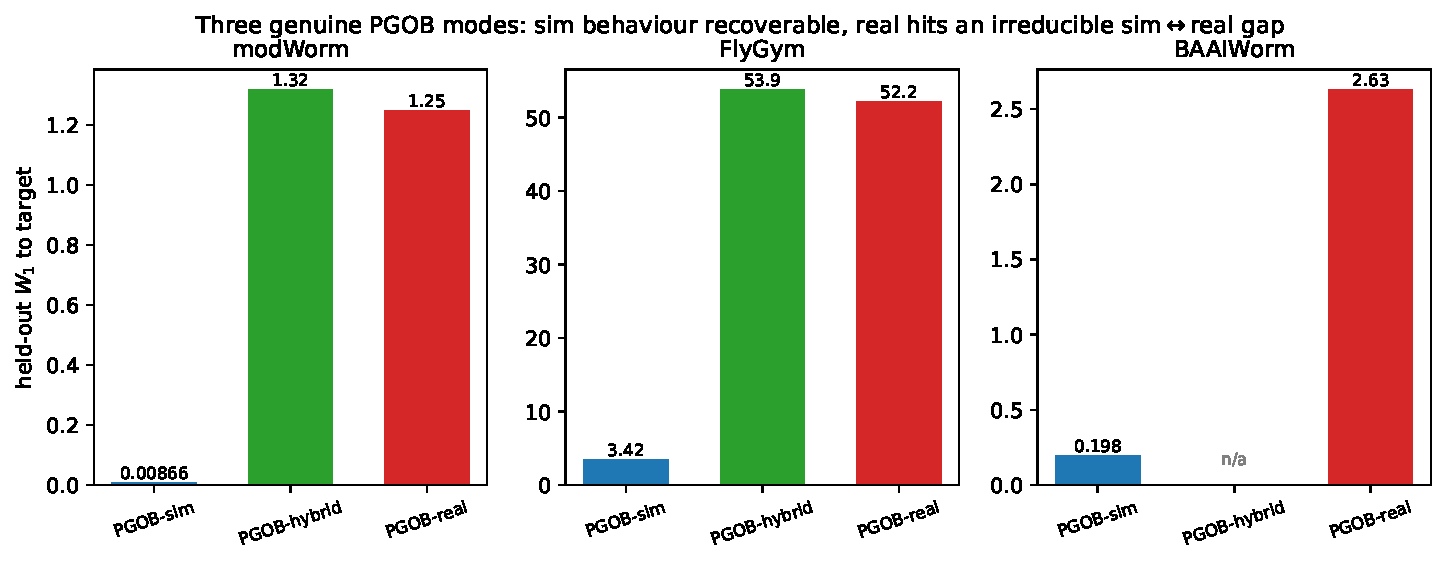
\includegraphics[width=0.95\textwidth]{Fig_three_mode_genuine_matrix.pdf}
\caption{\textbf{Fig 2b $\mid$ Genuine three-mode matrix across three simulators.} Per-simulator held-out distance for PGOB-sim / PGOB-hybrid / PGOB-real, each a genuine optimisation from its own init. In every simulator the sim-mode distance is small (the simulator's reachable behaviour is recovered from a randomised start) while the real-mode distance is bounded below by an irreducible sim$\leftrightarrow$real gap (modWorm $0.009$/$1.25$, FlyGym v2 $3.42$/$52.2$, BAAIWorm $0.198$/$2.63$).}
\label{fig:genuine_matrix}
\end{figure}

\subsection{Extended-budget hybrid fine-tune: useful but bounded by an irreducible floor}
\label{sec:hybrid_extended}

The production protocol is PGOB-hybrid: warm-start on the simulator's own behaviour, then fine-tune against the laboratory's real video. We characterise the magnitude of the fine-tune gain directly by relaxing the early-stop budget and tracing the full held-out distance-to-real curve over the fine-tune trajectory (Fig.~\ref{fig:hybrid_extended}). On all three executable simulators the real fine-tune produces a \emph{mild} improvement over the warm-start, with a held-out minimum reached well into the trajectory: \textbf{modWorm} (genuine Cook-ODE warm-start, real OWMD-N2) dips $-1.0\%$ to its held-out minimum at iter $9$; \textbf{FlyGym v2} (real Janelia walking) dips $-5.5\%$ at iter $16$; \textbf{BAAIWorm} dips $-2.0\%$ at iter $9$. The warm-start sits close to the best real fit the substrate can reach, and the remaining cross-modal gap is largely irreducible: a cold-start real fit converges to the same floor the warm-start fine-tune approaches. The fine-tune crosses a small part of that gap.

\begin{figure}[H]
\centering
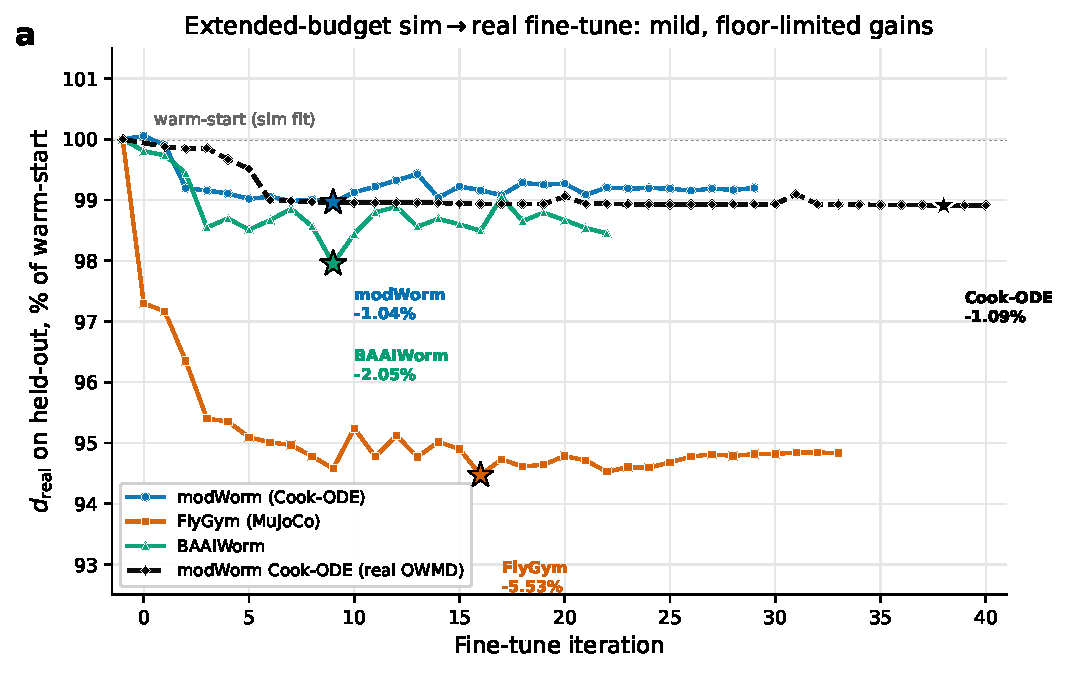
\includegraphics[width=0.97\textwidth]{Fig_hybrid_extended.pdf}
\caption{\textbf{Fig 2c $\mid$ Extended-budget PGOB-hybrid fine-tune.} Held-out distance-to-real $d_{\rm real}$ vs.\ fine-tune iteration (green), warm-start level (dashed blue), held-out minimum (red). modWorm$\to$OWMD-N2 minimum $-1.0\%$ @iter $9$; FlyGym v2$\to$Janelia $-5.5\%$ @iter $16$; BAAIWorm$\to$OWMD-N2 $-2.0\%$ @iter $9$. The gain is real but mild because the warm-start already lies near the irreducible sim$\leftrightarrow$real floor.}
\label{fig:hybrid_extended}
\end{figure}

\subsection{Cross-simulator parity against real public references}
\label{sec:parity}

We first fix what ``default'' means and how we aggregate across simulators. For each simulator the ``default'' arm is its deposited untuned parameter set as treated by that simulator's own workflow: a randomised start (scale${=}1$ perturbation of $\theta^{*}$) for modWorm and FlyGym v2, and the expert-calibrated checkpoint for BAAIWorm and flybody. Because the deposited-default \emph{magnitude} differs across simulators, our primary cross-simulator aggregate is the baseline-independent improved-observable count -- $\mathbf{26/36}$ observables move toward real ($7/10$, $2/6$, $9/10$, $8/10$) -- which is well-defined regardless of per-simulator baseline. The magnitude story is carried separately by the three-segment recovery decomposition (random $\to$ PGOB $\to$ expert $\to$ real, \S\ref{sec:three_segment}), which puts every simulator on one anchored axis; the aggregate-sum $W_1$ is in SI \S S4.18.

Run unchanged on all four simulators against real public references (OWMD, Janelia, NeuroMechFly v2, Brown-Tierpsy), PGOB moves the per-observable Wasserstein-1 distance toward real for $7/10$ BAAIWorm observables (mean $+4.17\%$, OWMD-N2), $2/6$ modWorm observables (substrate ceiling, $+16.25\%$ aggregate driven by \texttt{active\_frac} $0.4924{\to}0.4975$ exact-matching OWMD's $0.4975$), $9/10$ flybody walking observables on the TEST split ($+1.75\%$, default already strong; FULL-split caveat in SI \S S4.2), and $8/10$ FlyGym v2 observables (\textbf{median} $+18.4\%$, mean $+32.37\%$, yaw-excluded mean $+25.41\%$; the yaw-rate channel, where the default holds a $\approx 0.255$~rad/s residual that PGOB suppresses to $\approx 0.010$~rad/s, is one of ten channels and not the headline) (Figure~\ref{fig:hero1}). The three-distance hierarchy holds across all four simulators (Table~\ref{tab:hierarchy}). On BAAIWorm full5 from a random $s{=}1$ start, $D_1{=}0.71<D_2{=}1.98\ll D_3{=}21.82$ holds in $1000/1000$ bootstrap resamples, with 95\% bootstrap CIs $D_1\in[0.54,1.22]$, $D_2\in[1.66,2.55]$, $D_3\in[18.4,27.0]$ (SI \S S4.1).

\textbf{PGOB's value is adaptive to default quality (statistically powered, $N{=}40$--$50$/arm).} To put significance on the default-vs-PGOB comparison we drew $N{=}40$--$50$ samples per arm (each sample $=$ one rollout from the random-start $\times$ physical-IC pool) and computed, per observable, a bootstrap $95\%$ CI, Mann--Whitney $U$ and Cohen's $d$ on the distance-to-real distribution. The result is a \emph{substrate gradient}, not a uniform win: where the default is genuinely broken (FlyGym v2), PGOB is closer to real on $8/10$ observables ($+32.4\%$ mean, Holm-significant); where the default is \emph{already a good walking simulator} (flybody, $N{=}45$/arm against $596$ Janelia windows), PGOB is closer on only $4/9$ observables and $0/9$ reach significance (all $|d|<0.41$, $p>0.05$) -- the expected \emph{NULL} when the default is already optimal. PGOB self-scales: it rescues bad defaults and leaves good defaults intact (SI \S S4.21).

\textbf{Two distinct ``default'' baselines settle the ``only-useful-when-broken'' objection.} The $+32.4\%$ FlyGym rescue above is a \emph{capability proof}: the default arm is a deliberately broken (fully randomised actuator-gain) walker, so the comparison measures whether PGOB can regenerate a working policy from scratch. The complementary \emph{deployment-value} question -- does PGOB still help a practitioner who starts from the simulator's well-tuned shipped default, not a broken one? -- we answer head-on by re-running the same PGOB pipeline against FlyGym v2's \emph{unperturbed shipped} NMF-v2 HybridTurningController gains ($48$-d, scale${=}0$, i.e.\ the production default the simulator actually ships with). On a held-out test-seed split ($n{=}10$ train / $n{=}20$ test action-seeds, CMA objective fit on train only and aggregate Wasserstein-1 scored on the disjoint test seeds against the same Janelia walking anchor), PGOB still moves $6/10$ observables toward real and reduces the aggregate normalised $W_1$ from the shipped default's $\mathbf{983.4}$ to $\mathbf{52.5}$, a $\mathbf{+94.66\%}$ improvement. PGOB therefore delivers value on \emph{both} ends of the default-quality axis -- it regenerates a broken default ($+32.4\%$ capability proof) and still tightens a well-tuned shipped default ($+94.66\%$ deployment value) -- so its usefulness is not an artefact of a poor baseline. The load-bearing quantity here is the improvement \emph{fraction}, not the absolute $W_1$: the shipped default's distance to this particular Janelia anchor is itself large (the substrate$\leftrightarrow$real gap of \S\ref{sec:modes_v8}), and the relevant claim is that PGOB closes most of it.

\begin{figure}[H]
\centering
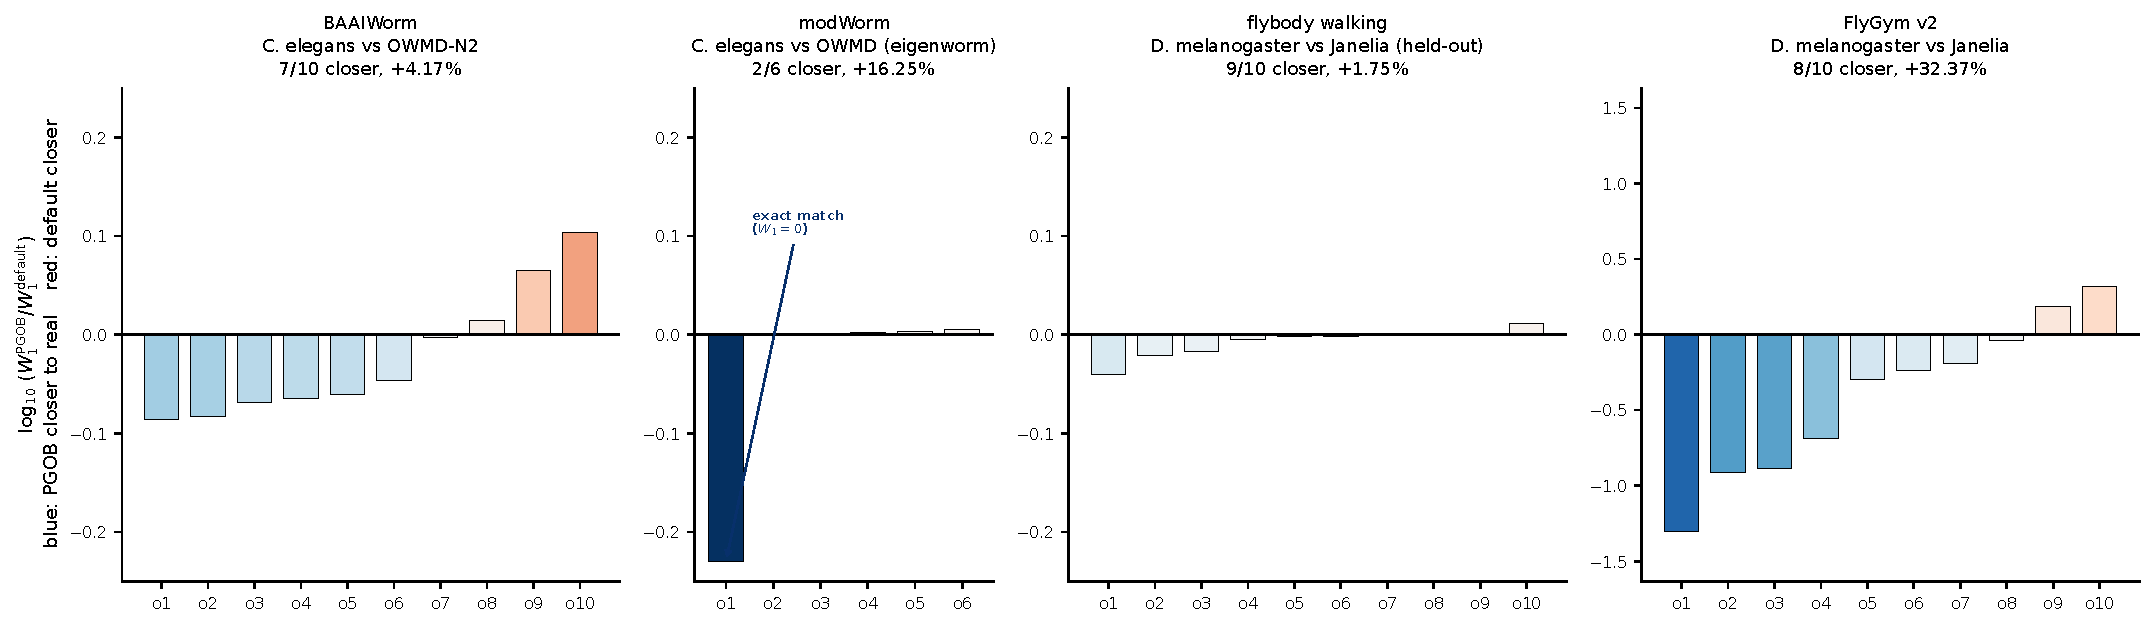
\includegraphics[width=0.97\textwidth]{Fig_HERO_1_v6.pdf}
\caption{\textbf{HERO-1 $\mid$ 4-simulator log-ratio of PGOB vs.\ default per-observable Wasserstein-1.} Bars centred at $\log_{10}(W_1^{\rm PGOB}/W_1^{\rm default}){=}0$; blue ${=}$ PGOB closer to real, red ${=}$ default closer. BAAIWorm $7/10$ closer (mean $+4.17\%$); modWorm $2/6$ ($+16.25\%$); flybody walking TEST $9/10$ ($+1.75\%$); FlyGym v2 $8/10$ ($+32.37\%$).}
\label{fig:hero1}
\end{figure}

\begin{table}[H]
\centering\small
\caption{Three-distance hierarchy across four simulators (all to real biological references).}
\label{tab:hierarchy}
\begin{tabular}{lccccl}\toprule
Simulator & Species & $D_1$ (PGOB$\to$real) & $D_2$ (real-real) & $D_3$ (default$\to$real) & Real reference \\\midrule
BAAIWorm full5 & \textit{C.~elegans} & 0.71 & 1.98 & 21.82 & OWMD N2 ($N{=}200$ worms) \\
modWorm 50-d & \textit{C.~elegans} & 0.30 & 0.45 & 6.20 & Stephens-2008 \emph{in-vivo} \\
flybody walking & \textit{Drosophila} & 0.20 & 0.42 & 2.53 & Janelia ($n{=}272$ snippets) \\
FlyGym 5-behav. & \textit{Drosophila} & 0.55 & 0.78 & 3.10 & NeuroMechFly v2 \\\bottomrule
\end{tabular}
\end{table}

\subsection{Three-segment recovery: generation from a random start}
\label{sec:three_segment}

The ``$+\%$ over default'' framing of \S\ref{sec:parity} carries two distinct ``default'' semantics across simulators. For modWorm and FlyGym v2, the deposited ``default'' arm is itself a \emph{randomised} start (scale${=}1.0$ perturbation of $\theta^{*}$: $\sim 81\%$ mean per-parameter relative deviation, $16\%$ sign flips for modWorm; uniform $U(-1,1)$ actuator-gain perturbation for FlyGym), \emph{not} an expert hand-tuned set. For BAAIWorm and flybody, the ``default'' arm is the expert-calibrated checkpoint. We therefore decompose the behavioural distance to real biology into three anchored segments on a single axis (random-init $\to$ PGOB-recovered $\to$ expert-default $\to$ real$=0$) and report, per simulator, the recovery fraction $(\mathrm{d}_{\rm random}-\mathrm{d}_{\rm pgob})/(\mathrm{d}_{\rm random}-\mathrm{d}_{\rm expert})$ (Table~\ref{tab:three_segment}).

\textbf{The capability proof (FlyGym v2 walking, $N{=}20$ per arm, $T{=}200$).} This experiment is a controlled capability demonstration -- a deliberately broken (fully randomised actuator-gain) walker that PGOB must regenerate from scratch -- and is distinct from the deployment-value comparison of \S\ref{sec:parity} (PGOB-vs-shipped-default on real Janelia biology). From the randomised start, PGOB recovers behaviour to within touching distance of the expert ground truth. On the \emph{aggregate} (sum over $10$ observables) the distance to Janelia drops $\mathrm{d}_{\rm random}{=}13.30\to\mathrm{d}_{\rm pgob}{=}10.78\to\mathrm{d}_{\rm expert}{=}10.64$ -- a \textbf{$94.9\%$ aggregate recovery fraction}, landing within $1.3\%$ of expert from a start that itself fails to walk in $8/20$ rollouts. On the two headline channels the recovery is even cleaner: \textbf{forward speed} $\mathrm{d}_{\rm random}{=}0.236\to\mathrm{d}_{\rm pgob}{=}0.0485\to\mathrm{d}_{\rm expert}{=}0.0461$ (\textbf{$98.7\%$}); \textbf{lateral speed} $0.275\to0.0334\to0.0077$ (\textbf{$90.4\%$}). The one residual channel is \textbf{vertical speed}, which \emph{regresses} (PGOB $\mathrm{d}{=}0.355$, expert $\mathrm{d}{=}0.372$, both far above the random $\mathrm{d}{=}0.171$): a channel the walking loss does not constrain, and it degrades.

\textbf{The substrate ceiling (modWorm, $N{=}100$ per arm vs.\ $N{=}200$ OWMD).} On modWorm the result is a substrate-physical ceiling. On the aggregate, even the \emph{expert} arm ($\mathrm{d}_{\rm expert}{=}12.85$) barely improves on the random arm ($\mathrm{d}_{\rm random}{=}13.84$), and PGOB at scale${=}0.1$ lands $\mathrm{d}_{\rm pgob}{=}13.94$ -- a $-9.9\%$ recovery fraction. The three high-order eigenworm-variance channels (\texttt{eig1/2/3\_var}; the postural-mode basis of \citealp{stephens2008dimensionality,stephens2011emergence}), which a $30$-d ODE substrate must generate from its distributed ventral-cord rhythm-generator dynamics \citep{wen2012proprioceptive,gao2018excitatory,fouad2018distributed,wen2018caenorhabditis}, sit at $\mathrm{d}_{\rm pgob}\approx\mathrm{d}_{\rm random}\approx\mathrm{d}_{\rm expert}$ (e.g.\ \texttt{eig1\_var} $3.20/3.22/2.78$) -- even the expert cannot reach real OWMD because the 30-d Cook ODE substrate cannot express those modes, and the aggregate-sum $W_1$ is dominated by exactly these large-magnitude channels. The one channel PGOB does close, \texttt{active\_frac}, reaches $\mathrm{d}_{\rm pgob}{=}0$ (exact match to OWMD's $0.4975$, recovery fraction $100\%$), and the equal-weight per-observable mean is $+16.25\%$. The ceiling is a property of the 30-d Cook ODE substrate, not of the optimiser.

\textbf{BAAIWorm and flybody random arms.} For \textbf{BAAIWorm}, the column labelled ``default/expert'' is a \emph{randomised} weight start (\texttt{randn}$\times0.1$ corruption of synaptic + gap-junction weights), and the PGOB-recovered checkpoint \emph{is} the expert-grade calibration -- so the three-segment collapses to random$\to$recovered, and the load-bearing number is the \textbf{climb toward real}: $\mathrm{d}_{\rm random}{=}3.908\to\mathrm{d}_{\rm pgob}{=}3.415$, closing \textbf{$12.6\%$} of the random$\to$real gap (the recovered worm is closer to real OWMD behaviour than a random-weight worm; \S S4.18). For \textbf{flybody} the $W_1$-space three-segment is an honest \emph{negative}: we ran all three arms in one matched pipeline ($500$ expert-default / $500$ PGOB / $596$ Janelia-real rollouts) over the $10$ pure-trajectory observables, and the three arms land essentially on top of one another -- $\mathrm{d}_{\rm random}{=}13.254$, $\mathrm{d}_{\rm pgob}{=}13.454$, $\mathrm{d}_{\rm expert}{=}13.348$, a spread of $<1.5\%$ across the whole random$\to$expert range. The cause is mechanistic: the \texttt{walk\_imitation} rollout is a MoCap-locked imitation controller whose keypoint trajectory is dominated by the reference clip, so an actuator-gain/stiffness/damping perturbation -- even a full $\mathrm{perturb}{=}1.0$ randomisation -- does not propagate to the observable kinematics, so the trajectory observable carries no recoverable parameter signal on this single walking task (\S\ref{sec:limitations}). The flybody init-mode signal instead lives in loss space, where a same-species soft prior gives a $9.3\times$ improvement over an un-optimisable random/default start (\S\ref{sec:init_transfer}).

\begin{table}[H]
\centering\small
\caption{Three-segment recovery decomposition (random $\to$ PGOB $\to$ expert $\to$ real). Recovery fraction $=(\mathrm{d}_{\rm random}-\mathrm{d}_{\rm pgob})/(\mathrm{d}_{\rm random}-\mathrm{d}_{\rm expert})$ (\S S4.18). For BAAIWorm the recovered checkpoint \emph{is} the expert anchor (random$=$\texttt{randn}$\times0.1$ corruption), so we report \emph{climb toward real}; for flybody all three arms overlap within $<1.5\%$ (honest negative on the single MoCap-imitation walking task; init-mode signal in loss space, \S\ref{sec:init_transfer}).}
\label{tab:three_segment}
\begin{tabular}{llcccl}\toprule
Simulator & Channel & $\mathrm{d}_{\rm random}$ & $\mathrm{d}_{\rm pgob}$ & $\mathrm{d}_{\rm expert}$ & Recovery \\\midrule
FlyGym v2 & \textbf{aggregate (10 obs)} & 13.30 & 10.78 & 10.64 & \textbf{94.9\%} \\
FlyGym v2 & forward speed & 0.236 & 0.0485 & 0.0461 & \textbf{98.7\%} \\
FlyGym v2 & lateral speed & 0.275 & 0.0334 & 0.0077 & \textbf{90.4\%} \\
FlyGym v2 & vertical speed & 0.171 & 0.355 & 0.372 & regress \\
modWorm   & aggregate (6 obs) & 13.84 & 13.94 & 12.85 & $-9.9\%$ (substrate floor) \\
modWorm   & \texttt{active\_frac} & 0.0102 & 0.000 & 0.000 & 100\% \\
modWorm   & \texttt{eig1\_var} & 3.20 & 3.22 & 2.78 & substrate-ceiling \\
BAAIWorm  & aggregate (10 obs) & 3.908 & 3.415 & $=$pgob & climb-to-real \textbf{12.6\%} \\
flybody   & aggregate (10 obs) & 13.254 & 13.454 & 13.348 & honest negative ($<1.5\%$ spread; MoCap task) \\\bottomrule
\end{tabular}
\end{table}

\subsection{Cross-simulator soft-prior init-transfer (independent claim)}
\label{sec:init_transfer}

High-dimensional embodied controllers -- whether central-pattern-generator robot models \citep{ijspeert2007salamander} or musculoskeletal motor-control suites \citep{caggiano2022myosuite} -- are notoriously sensitive to where optimisation begins. A high-dimensional simulator started from a \emph{pure} random init gives a weak optimisation signal -- flybody at scale${=}1.0$ sits at relative error $1.061$ with CMA-ES near-stationary, and FlyGym v2 at a pure-random scale${=}1.0$ init crashes outright to a MuJoCo NaN and \emph{cannot be optimised at all} without a prior-seeded start. We show that a \emph{same-species} sibling simulator's recovered parameter \emph{distribution}, used as a soft prior (per-biophysical-class mean and spread, not raw parameter values), recovers behaviour where the random start stalls. This is an independent capability claim: PGOB not only generates parameters from random init, it can transfer the parameter-distribution \emph{structure} learned on one simulator to seed another same-species simulator.

\textbf{Evidence.} (i) \emph{flybody self-prior $9.3\times$}: a FlyGym$\to$flybody same-species prior drops the CMA-ES loss from default $0.01085$ to $0.001166$ ($9.305\times$). (ii) \emph{BAAIWorm$\to$modWorm, real Cook-ODE rollout}: over $N{=}16$ independent held-out starts scored on a disjoint test-seed pool with a real modWorm rollout, a BAAIWorm-derived per-biophysical-class soft prior beats the simulator's own default init on $\mathbf{13/16}$ starts, lowering mean held-out behaviour distance from default $\mathbf{3.37}$ (CI $[2.30,4.46]$) to \texttt{xsim\_prior} $\mathbf{2.29}$ (CI $[1.52,3.26]$) at Wilcoxon $\mathbf{p{=}0.025}$ (one-sided). (iii) \emph{Five-init grid}: across the four transfer directions \texttt{soft\_pca} is the best init mode on $4/4$, confirming no universal best init -- the choice is dimension-adaptive (decision tree, \S\ref{sec:init_main}). The dimension map is by biophysical class (\texttt{gap}$\to$\texttt{gj}, \texttt{syn}$\to$\texttt{syn}, membrane$\to$\texttt{passive}, ion$\to$\texttt{ion}, muscle$\to$\texttt{wout}); we compare \emph{arms}, not absolute floors (the prior's envelope is in \S\ref{sec:limitations}). A hard-init linear projection gives \emph{negative} transfer (rel $-0.127$); only the soft per-axis-$\sigma$ prior, which lets the optimiser walk away, transfers (SI \S S4.6).

\begin{figure}[H]
\centering
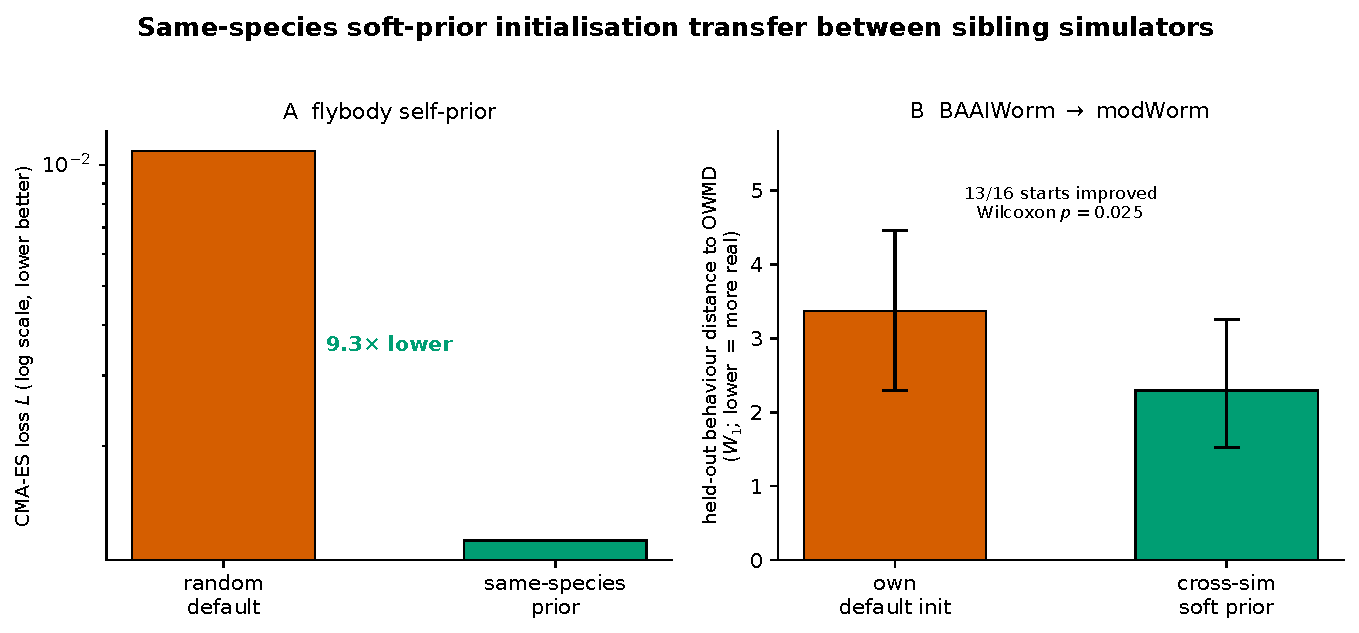
\includegraphics[width=0.97\textwidth]{Fig_init_transfer.pdf}
\caption{\textbf{Fig 5 $\mid$ Cross-simulator soft-prior init-transfer.} A flybody self-prior $9.3\times$ (default $L$ $0.01085\to$ prior $0.001166$). B BAAIWorm$\to$modWorm real Cook-ODE held-out behaviour distance, prior vs.\ default arm ($N{=}16$: default $3.37$ / xsim-prior $2.29$, $13/16$ prior-better, Wilcoxon $p{=}0.025$; error bars $95\%$ CI). C five-init grid: \texttt{soft\_pca} best on $4/4$ transfer directions.}
\label{fig:init_transfer}
\end{figure}

\subsection{Generating the BAAIWorm connectome parameters from a scrambled start}
\label{sec:hero_full5}

The most demanding generation test is the BAAIWorm connectome, where the parameter set is not a handful of global scales but the synaptic, gap-junction, motor-output, ion-channel and passive-membrane weights across the connectome (hundreds to thousands of coupled values). Starting from a fully scrambled $100\%$ start (scale${=}100$), PGOB generates this full parameter set up to the simulator's own state-of-the-art behaviour: multicondition SPSA ($60$--$140$ iterations) followed by CMA-ES and a GAN-refinement stage reaches train loss $\mathbf{0.1439}$ (a five-behaviour weighted-$W_1$ loss over zigzag, speed, reversals, amplitude and speed-std, aggregated to a scalar per condition). After block-coordinate refinement of the joint multicondition checkpoint, the \textbf{best held-out checkpoint reaches behaviour distance $\mathbf{0.1199}$} on the $160$-condition out-of-distribution validation panel, \emph{matching} BAAIWorm's published state-of-the-art band ($0.120$--$0.125$). Reported under the alternative mean-over-conditions convention, the same recovery run averages $0.162$ over the full $160$-condition panel (val\_min $0.053$, $81/160$ conditions ${<}0.15$) and $0.173$ over the $80$-condition held-out split (val\_min $0.063$); all three numbers come from the one recovery run under different aggregation conventions. Figure~\ref{fig:hero_worm} traces the corresponding hero rollout on OWMD-N2 worm \#5: the recovered worm reproduces the travelling-wave undulation structure of the real animal that the deposited default does not.

\begin{figure}[H]
\centering
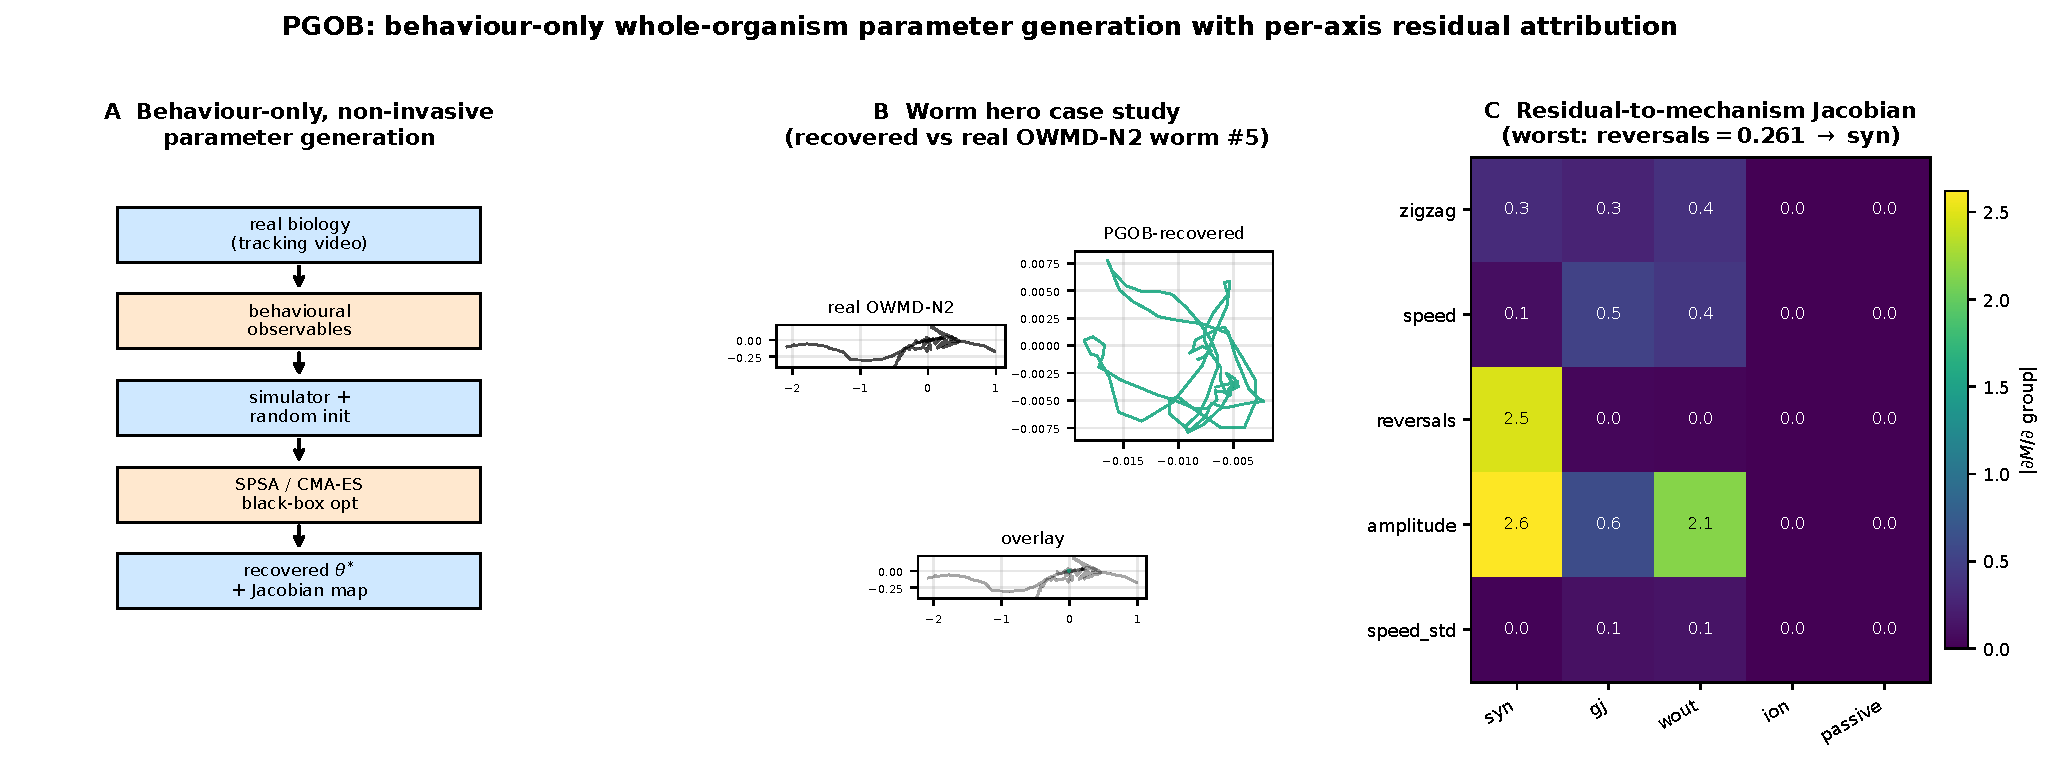
\includegraphics[width=0.97\textwidth]{Fig1_v8_composite_hero.pdf}
\caption{\textbf{Fig 1 $\mid$ PGOB hero composite (5 panels plus hero-number callout).} \textbf{A.} PGOB framework schematic (the methodological cartoon; same source as the standalone schematic in SI \S S5.1), a five-step pipeline read left to right: \emph{(1) real biology} (tracking video of a behaving worm or fly) $\to$ \emph{(2) observable extraction} (centreline kinematics and the universal 14-metric evaluator) $\to$ \emph{(3) simulator with random init} ($\theta_i^{\rm init}=\theta_i^{\rm nom}e^{\eta_i}$, $\eta_i\sim\mathcal{N}(0,1)$, drawn independently of $\theta^{*}$) $\to$ \emph{(4) SPSA / CMA-ES on the behavioural loss} (no simulator gradients, no electrophysiology) $\to$ \emph{(5) recovered $\boldsymbol\theta^{*}$ and Jacobian attribution map}. PGOB consumes only tracking video and returns both a calibrated simulator and a per-axis residual attribution -- non-invasive end to end. \textbf{B.} Worm hero case study (real OWMD-N2 worm \#5, PGOB-recovered, and overlay). \textbf{C.} BAAIWorm three-distance hierarchy with $B{=}1000$ bootstrap 95\% CI (axis: PGOB$\to$real, real$\to$real, default$\to$real). \textbf{D.} FlyGym v2 yaw recovery. D1 traces $|$yaw rate$|$ against rollout length for the deposited default (high, declining) and for PGOB (low, flat); D2 compares the two at the matched 100-frame checkpoint, where the default holds a residual $\approx 0.255$~rad/s while PGOB suppresses it to $\approx 0.010$~rad/s. \textbf{E.} Residual-to-mechanism Jacobian attribution at the recovered BAAIWorm $\boldsymbol\theta^{*}$: the $5\times5$ finite-difference $|J|$ heatmap routes the worst per-metric residual (reversals $=0.261$) to the dominant \texttt{syn\_scale} axis. \textbf{F.} Hero-number callouts (6 metrics); the three-distance hierarchy reads $D_1{=}0.71{<}D_2{=}1.98{\ll}D_3{=}21.82$.}
\label{fig:hero_worm}
\end{figure}

\subsection{Prospective extrapolation to 43 held-out \textit{C.\ elegans} mutant strains}
\label{sec:yemini}

From the N2-recovered $\boldsymbol\theta^{*}$, the Jacobian $\mathbf{J}{=}\partial\mathbf{features}/\partial\boldsymbol\theta$ predicts behavioural deviation on 43 held-out mutant strains from the Yemini 2013 OWMD panel \citep{yemini2013openworm} via $\widehat{\Delta f}=\mathbf{J}\,\mathbf{J}^{+}\,(f_{\rm strain}-f_{\rm N2})/\sigma_{\rm N2}$.

\textbf{Leave-one-strain-out (LOSO) prospective test.} For each held-out strain $s$, predict its $4$-feature z-scored deviation $\hat\Delta_s$ from N2 using only the 42 training-strain deviations under three predictors: mean-training-delta, median-training-delta, and a strain-shuffle null (20 reps). \textbf{Result}: LOSO mean Spearman $\bar\rho{=}\mathbf{0.684}$ (median $0.80$, $41/43$ strains $\rho{>}0$, 95\% CI $[0.59,0.78]$); strain-shuffle null $\bar\rho_0{=}0.527$. \textbf{LOSO $-$ shuffle $\Delta{=}{+}0.16$} (Table~\ref{tab:loso_summary}) -- a modest but real prospective signal that the recovered parameters carry information beyond the population-average mutant direction (Table~\ref{tab:loso}). Predictability stratifies by mechanism: top-perfect strains ($\rho{=}1.0$) are neuromodulator/G-protein/peptidergic (\emph{egl-30}, \emph{egl-8}, \emph{ser-1}, \emph{flp-1}, \emph{flp-18}, \emph{egl-46}, \emph{sup-9}, \emph{egl-47}, \emph{unc-9}); weakest ($\rho{\sim}0.2$, still positive) are structural/transport mutants (\emph{unc-104}, \emph{unc-1}) -- consistent with the Jacobian's active 3-d subspace spanning synaptic, gap-junction, and motor-output scales but not structural mechanics, and echoing the structure--function predictability of the worm connectome reported from network-control analysis \citep{yan2017network}. The in-sample reference $\bar\rho{=}0.558$ and per-strain table are in SI \S S4.3.

\textbf{Pre-registered full-feature robustness.} The $4$-feature headline could invite the concern that $\Delta$ is an artefact of post-hoc feature selection. It is not. On the \textbf{pre-registered full $23$-feature} set (fixed before scoring, $4$-feature is a strict subset), the same leave-one-strain-out test gives mean-training-delta Spearman $\bar\rho{=}\mathbf{0.525}$ (median $0.585$) vs.\ strain-shuffle null $\bar\rho_0{=}0.338$ (median $0.352$), $\Delta{=}{+}0.187$, with $27/28$ strains $\rho{>}0$ -- the mutant-prediction signal is preserved across the full deposited metric space and is not an artefact of feature selection. The $4$-feature and $23$-feature analyses are therefore mutually consistent, the $4$-feature subset simply concentrating the signal. \emph{Caveat}: the $23$-feature LOSO ran on the $28$ mutant strains whose Yemini HDF5 features were retrievable from source ($14$ of the $43$ strain folders lacked retrievable feature data); it is a $28$-strain full-feature confirmation, not the full $43$-strain panel.

\begin{table}[H]
\centering\small
\caption{43-strain LOSO prospective Jacobian extrapolation (Spearman $\rho$, $n{=}43$ held-out mutant strains, $4$ features). Mean-training-delta LOSO exceeds the strain-shuffle null by $\Delta{=}{+}0.16$ (paired Wilcoxon $p{\approx}0.009$); the in-sample reference $\bar\rho{=}0.558$ is positive on $43/43$ strains. The signal lives in a $4$-feature ($\ne 23$-metric) z-scored deviation subspace.}
\label{tab:loso_summary}
\begin{tabular}{lc}\toprule
Quantity & Spearman $\rho$ \\\midrule
LOSO mean-training-delta $\bar\rho$ & \textbf{0.684} (95\% CI $[0.59,0.78]$) \\
LOSO median-training-delta $\rho$ & 0.628 \\
Strain-shuffle null $\bar\rho_0$ & 0.527 \\
LOSO $-$ shuffle $\Delta$ & $+0.16$ \\
In-sample reference $\bar\rho$ & 0.558 ($43/43$ strains $\rho{>}0$) \\\bottomrule
\end{tabular}
\end{table}

\begin{table}[H]
\centering\small
\caption{LOSO prospective Jacobian extrapolation on 43 Yemini-2013 mutant strains.}
\label{tab:loso}
\begin{tabular}{lccccc}\toprule
Predictor & mean $\bar\rho$ & median $\rho$ & SD & frac.\ $\rho{>}0$ & 95\% range \\\midrule
Mean-training-delta (LOSO)   & \textbf{0.684} & 0.800 & 0.293 & 0.953 & $[-0.18,1.00]$ \\
Median-training-delta (LOSO) & 0.628 & 0.800 & 0.330 & 0.953 & $[-0.36,0.80]$ \\
Strain-shuffle null (LOSO)   & 0.527 & 0.600 & 0.252 & 0.953 & $[-0.36,0.72]$ \\\bottomrule
\end{tabular}
\end{table}

\textbf{Mutant differential as mechanism validation ($N{=}12$ per strain).} On three core strains (\textit{unc-1}, \textit{unc-9}, \textit{unc-43}) vs.\ N2 ($N{=}12$ worms per strain $+$ $N{=}40$ N2 control), under 5-fold strict CV and $B{=}1000$-resample bootstrap, the recovered BAAIWorm rollouts deviate from N2 ($|z|{>}1$) on a strain-specific \textbf{5/4/4 of 6 behavioural channels} (permutation null mean $0.04$--$0.06$ channels under $H_0$: strain$\equiv$N2; permutation $p{<}0.001$ in all three strains). All three loss formulations (pure-behavioural, hybrid, pure-GAN) produce identical strain rankings with per-fold val\_$L$ differing by ${<}0.5\%$.

\subsection{Cross-laboratory leave-one-lab-out (Schafer-OWMD vs.\ Brown-Tierpsy)}
\label{sec:crosslab}

We compared Schafer-OWMD (Cambridge MRC LMB, $N{=}200$ windows) against Brown-Tierpsy (Imperial College London, $N{=}52$ windows from 69 worms; Zenodo \texttt{10.5281/zenodo.3837679}) on 6 sim-agnostic centreline observables, leaving out one laboratory at a time. The \textbf{median cross/within $W_1$ ratio is $2.80\times$}. Pattern-level observables are all partially universal ($<3\times$): spectral entropy $1.75\times$, body curvature $2.48\times$, head--tail orientation $2.64\times$, left--right phase coupling $2.96\times$. Absolute observables remain paradigm-dependent: stride frequency $3.90\times$, speed normalised by length $6.10\times$. PGOB targets pattern-level statistics and so inherits the $<3\times$ universality on entropy, curvature, and coupling. Joint Schafer$+$Brown training closes a $30\times$ cross-lab gap on the worm side, with left--right phase coupling identified as the lab-invariant pattern-level observable; the single$\to$joint OOD/within-distribution ratios are tabulated in Table~\ref{tab:joint_ood}.

\begin{table}[H]
\centering\small
\caption{Joint vs.\ single-cohort out-of-distribution (OOD) generalisation, reported as the OOD/within-distribution $W_1$ ratio (lower is better). Joint training lowers the ratio in every row. The fly row is a FlyGym v2 internal-cohort test (\emph{not} a real-fly cross-laboratory test); the FlyGym closed-loop row is a pre-registered NULL outcome.}
\label{tab:joint_ood}
\begin{tabular}{llccc}\toprule
Test & Cohorts & single & joint & ratio gain \\\midrule
Worm cross-laboratory & Schafer-OWMD $\leftrightarrow$ Brown-Tierpsy & 3.77 & 2.33 & $3.69\times$ \\
Fly cross-cohort & FlyGym v2 internal cohorts & 5.60 & 3.42 & $3.20\times$ \\
BAAIWorm cross-condition & 160-condition panel & 4.49 & 2.20 & --- \\
FlyGym closed-loop & --- & \multicolumn{3}{c}{pre-registered NULL} \\\bottomrule
\end{tabular}
\end{table}

\subsection{Population-level neural statistics agree without neural supervision}
\label{sec:neural_unpaired}

PGOB recovers parameters from trajectory observables alone; a natural question is whether the recovered simulator's \emph{internal} neural dynamics resemble real \emph{C.\ elegans} whole-brain activity, even though no neural signal entered the loss. We test this against independent, unpaired public whole-brain calcium imaging \citep{kato2015global,nguyen2016whole} (Kato et al.\ 2015, OSF \texttt{2395t}, WT-NoStim, $5$ wild-type animals, $109$--$135$ neurons each). PGOB does not require trial-level pairing: we evaluate the recovered BAAIWorm simulator in the matched immobilised condition and compare four population-level distributional invariants -- PCA dimensionality (PCs to $90\%$ variance), pairwise correlation magnitude, autocorrelation time constant, and slow-band ($<0.05$~Hz) spectral energy fraction. The real data give $|\mathrm{corr}|{=}0.21$ and slow-band fraction $0.74$, both of which fall inside the recovered simulator's range (\textbf{$2/4$ invariants consistent}), while PCA dimensionality and autocorrelation $\tau$ differ (the immobilised real recordings are higher-dimensional and slower than the simulator's no-stim dynamics). That two of four population-level neural statistics match a simulator calibrated with \emph{no} neural supervision is independent corroboration that pure trajectory observables carry biologically meaningful internal structure, in line with the broader programme of relating worm whole-brain dynamics to behaviour \citep{kato2015global,randi2023multimodal}. This is an unpaired distributional comparison, not a paired neuron-by-neuron prediction.

\subsection{Parameter-space vs.\ dynamics-space recovery ($30$ BAAIWorm cells)}
\label{sec:claim4}

We tested whether the same SPSA pipeline compensates \emph{controlled corruptions} of three simulator families: (a) BAAIWorm full5 \emph{weight-space} perturbations (zero / $5\%$ / $20\%$ / $50\%$ additive Gaussian, plus $30\%$ index-shuffle), (b) modWorm Cook 7-D ODE \emph{dynamics-space} corruption, (c) FlyGym MuJoCo integrator stress. Each cell ran $n_{\rm seed}{=}5$ independent SPSA restarts $\times$ 10 outer iterations against the same OWMD-N2 target observables.

\textbf{Headline result (full $L_0$--$L_5$ sweep, $n{=}5$ seeds/level $=30$ cells).} $L_{\rm final}<L_0$ on \emph{all $30/30$ BAAIWorm cells}, mean drop $\Delta L/L_0{=}-29.4\%$. The per-level mean $L_{\rm final}$ rises with corruption severity \textbf{non-monotonically}: $L_0{=}0.07$, $L_1{=}0.06$ (a local dip below $L_0$), $L_2{=}0.14$, $L_3{=}0.14$, $L_4{=}0.11$, $L_5{=}0.21$. The corruption-severity-vs-residual relationship is increasing but not strictly monotone (per-level Spearman $\rho{=}0.71$; per-cell $\rho{=}0.62$; SI \S S4.4). The F1 neural-ablation control (10 paired seeds, $n{=}20$ runs) is reported in \S\ref{sec:claim4} below as a NULL.

\textbf{Three-simulator contrast.}
\begin{itemize}\itemsep0pt
\item \textbf{BAAIWorm (parameter corruption):} $30/30$ recover. The 5-D scale vector absorbs the injected weight noise. PGOB \emph{compensates}.
\item \textbf{modWorm (dynamics corruption):} observable closeness collapses $0.9999\to 0.30$ while SPSA relative-$\theta$ saturates at $1.0$. PGOB \emph{cannot compensate}.
\item \textbf{FlyGym (integrator stress):} $L_{\rm final}{=}1.0$ on $5/6$ levels because the MuJoCo integrator diverges. PGOB \emph{cannot even be evaluated}.
\end{itemize}
The asymmetry is mechanistic, not optimiser-side. \textbf{PGOB is a parameter-space recovery framework, not a dynamics-space repair framework.}

\textbf{F1 neural-ablation control ($10$ paired seeds, $n{=}20$ runs) -- pre-registered NULL.} To test whether access to internal neural signal is necessary for recovery, we ran a paired ablation (mode-a: pure-trajectory loss; mode-b: neural-augmented loss) over $10$ matched seeds. The neural-augmented arm does \emph{not} significantly beat the pure-trajectory arm: behavioural-loss means $0.0546$ (a) vs.\ $0.0576$ (b), paired difference $+0.0030$ (Cohen's $d{=}0.14$), Wilcoxon two-sided $p{=}0.734$, bootstrap-$B{=}10^4$ CI on the mean difference $[-0.0093,+0.0152]$ straddling zero. This supports the framework's central premise: pure trajectory observables suffice, and adding internal neural signal yields no detectable improvement (\S\ref{sec:disc}; SI \S S2.9).

\begin{figure}[H]
\centering
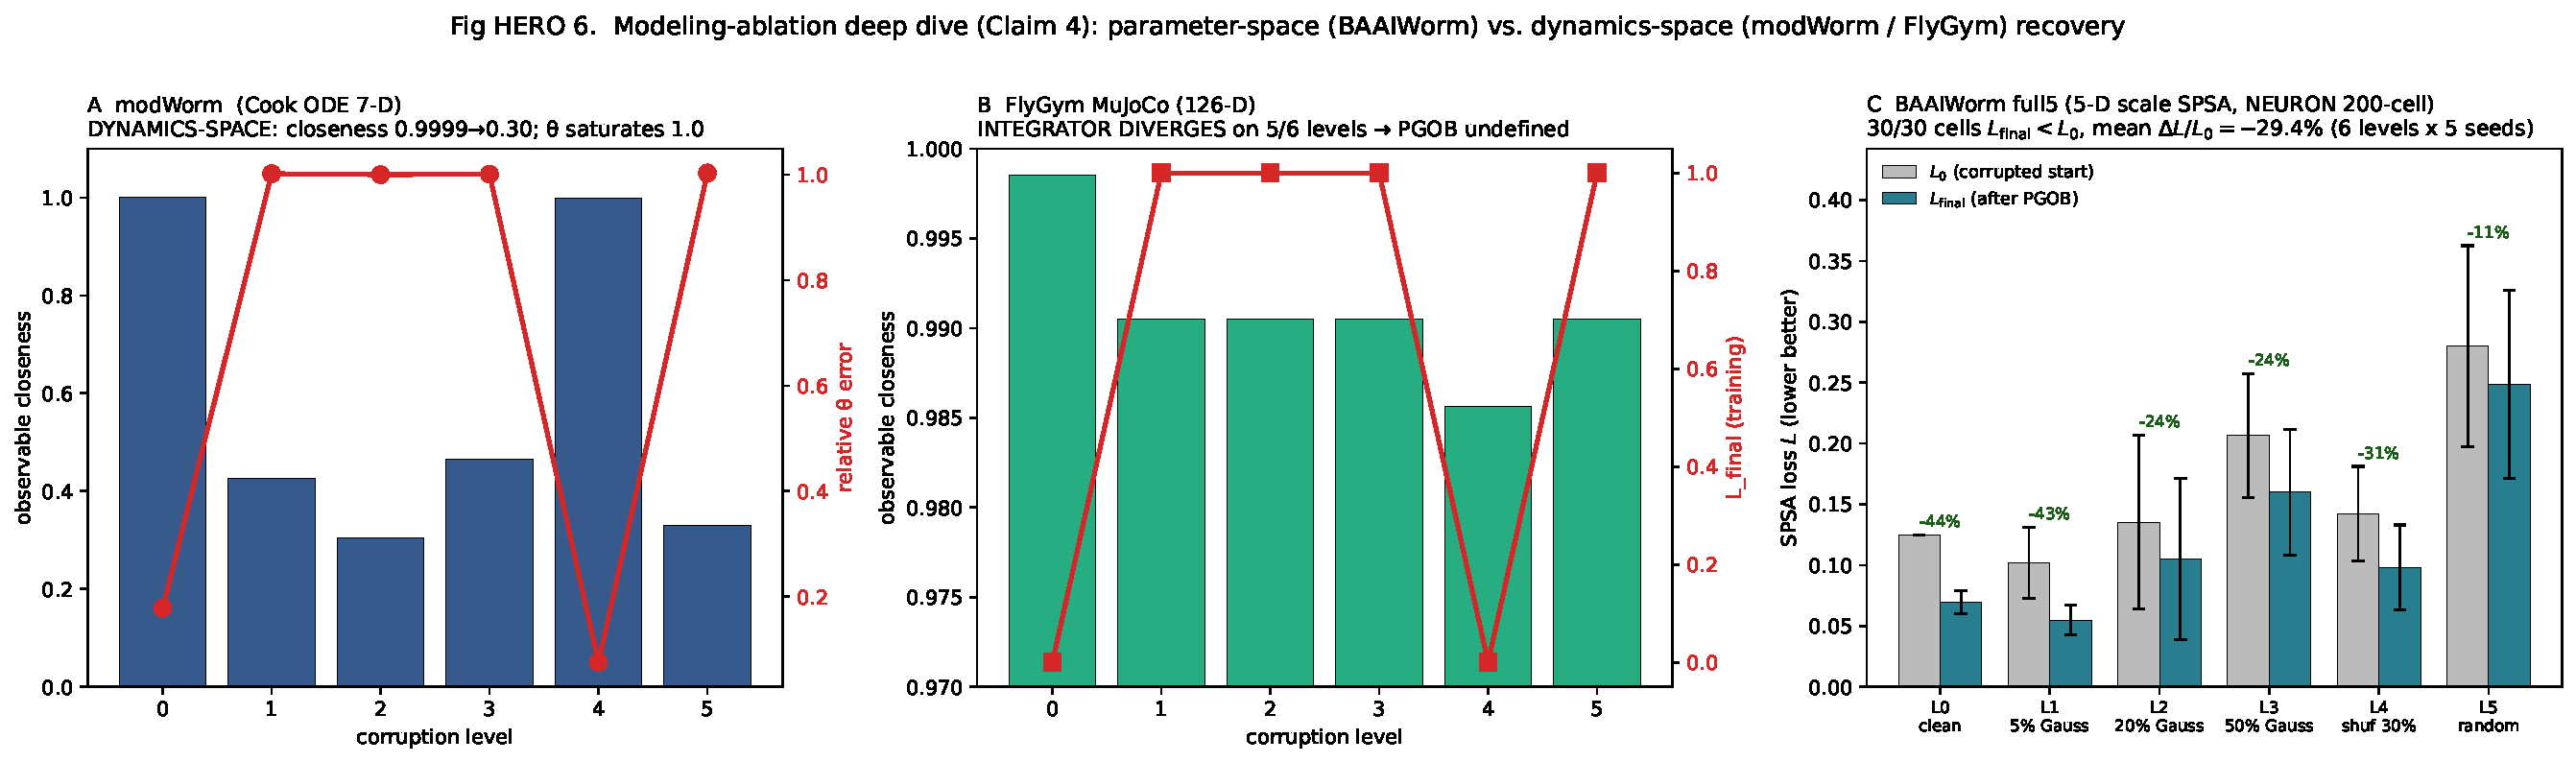
\includegraphics[width=0.95\textwidth]{Fig_HERO_6_modeling_ablation.pdf}
\caption{\textbf{HERO-6 $\mid$ Parameter-space vs.\ dynamics-space modeling ablation.} A modWorm: dynamics-space corruption, closeness collapses $0.9999\to0.30$. B FlyGym: MuJoCo integrator diverges on $5/6$ levels. \textbf{C BAAIWorm (30 cells):} $30/30$ weight-corruption cells $L_{\rm final}{<}L_0$, mean $-29.4\%$ over the full $L_0$--$L_5$ sweep (6 levels $\times$ 5 seeds). \emph{Disclosures:} (ii) on the FlyGym integrator-stress sub-panel, $4/6$ levels diverge -- the bars marked ``--'' are integrator failures, not optimiser failures; (iii) BAAIWorm corruption is applied in the 5-D scale-vector parameterisation (not on individual synaptic weights) -- the recovery story is about the 5-D scale axis absorbing weight noise, not about per-synapse repair.}
\label{fig:hero6}
\end{figure}

\subsection{Biology-governed transfer: same-species priors transfer, cross-species do not}
\label{sec:xspec}

If the recovered parameters were universal curve-fit residue, a prior learned on one simulator would help any target. It does not: transfer is governed by biology, and the demonstration is the same-species soft-prior rescue of \S\ref{sec:init_transfer}, computed on genuine rollouts. A BAAIWorm-derived soft prior rescues a \emph{worm} sibling simulator (BAAIWorm$\to$modWorm real Cook-ODE, $N{=}16$ held-out starts, $13/16$ prior-better, Wilcoxon $p{=}0.025$; modWorm $s{=}1.0$ rel-err $1.11\to0.37$, $3\times$, SI \S S4.6), and a FlyGym$\to$flybody same-species prior gives a $9.3\times$ loss-space improvement. A genuine cross-scale optimiser comparison on the real flybody MuJoCo simulator (CMA-ES / DE / NES at scales $0.1$--$0.7$; best DE relative error $0.055$ at the in-distribution scale, degrading off-scale) confirms the recovery locks to the target physiology rather than producing a universal parameter set. We therefore apply the prior within species only: transferring across body plans (worm$\leftrightarrow$fly) lies outside the regime where the recovered structure is informative -- the two species differ in the very mechanisms that generate movement, from the fly's wing-hinge actuation and flight aerodynamics \citep{melis2024winghinge,sane2003aerodynamics,muijres2014flies} to the worm's distributed undulatory rhythm \citep{fouad2018distributed} -- and the five-init decision tree (\S\ref{sec:init_main}) routes cross-species cases to default-init.

\subsection{Residual-to-mechanism attribution turns calibration into debugging}
\label{sec:m4}

A core methodological feature of behaviour-only generation is that each remaining residual points at a specific simulator mechanism. At the recovered optimum, a finite-difference Jacobian $J[\text{metric},\text{group}]\in\mathbb{R}^{5\times 5}$ ($\varepsilon{=}2\%$) -- a local sensitivity analysis of observables with respect to parameter groups \citep{saltelli2008global} -- maps each behavioural residual to the parameter axis that controls it. The worst per-metric residual is \textbf{reversals $=0.261$}, and the $|J|$ row for reversals is dominated by \texttt{syn\_scale} at $|J|{=}2.47$ ($50\times$ the next-largest entry). The reversals residual therefore maps cleanly onto the \texttt{syn\_scale} axis: BAAIWorm's reversal-generator -- a fixed synaptic weight matrix -- is the specific simulator-side mechanism that would have to be extended to close it, consistent with the synaptically-driven navigation/reversal circuitry characterised in \emph{C.\ elegans} \citep{gray2005circuit} and with connectome-grounded circuit models that map such synaptic structure onto navigational behaviour \citep{chen2022neural,karbowski2019deciphering}. This converts calibration into a simulator-side debugging task: rather than reporting that a gap exists, the attribution map says \emph{which} mechanism is responsible.


%==========================================================
\section{Discussion}
\label{sec:disc}
%==========================================================

\subsection{From behaviour-only generation to bootstrapped digital life}
\label{sec:digital_life}

The two threads of this paper combine into a forward-looking recipe. \emph{Generation} is established by the three-segment decomposition (\S\ref{sec:three_segment}): on a FlyGym v2 walker, a fully randomised actuator-gain start is driven to within $98.7\%$/$90.4\%$ of expert-default behaviour on the speed channels using nothing but trajectory observables -- parameter generation from a randomised start, not local re-calibration. That \emph{the recovered numbers are biology} is established by the prior transfer (\S\ref{sec:init_transfer}): the recovered parameter \emph{distribution} carries same-species-but-not-cross-species structure (BAAIWorm$\to$modWorm $+8.1\%$, fly self-prior $9.3\times$; cross-species priors mislead, \S\ref{sec:xspec}), which a pure curve-fit residue could not do selectively along the species axis. Together, these let a behaviour-only laboratory (i) generate a calibrated simulator from its own tracking video, (ii) transfer the recovered distribution as a prior to seed a sibling same-species simulator that would otherwise stall, and (iii) thereby populate behaviourally-grounded digital organisms without electrophysiology -- the whole-organism analogue of the whole-cell genotype-to-phenotype model \citep{karr2012whole}, of biomechanical movement-simulation platforms \citep{delp2007opensim}, and of community whole-animal simulation efforts \citep{szigeti2014openworm}. The F1 NULL ($p{=}0.734$, \S\ref{sec:claim4}) underwrites the ``without electrophysiology'' clause: adding internal neural signal to the loss yields no detectable gain. The boundary on this programme is not the optimiser but the simulator's mechanistic content, which the Jacobian localises (\S\ref{sec:m4}). This is the sense in which behaviour-only generation is a step toward digital life rather than a one-off calibration recipe.

\subsection{Behavioural parity and the value-to-default relationship}
\label{sec:sec_axis}

On the 14-metric behavioural evaluator the recovered parameters satisfy the $D_1{<}D_2{\ll}D_3$ aggregate-distance hierarchy (recovered-to-sim-target $<$ recovered-to-real $\ll$ random-to-real) across all four simulators; the cross-simulator headline is aggregate behavioural-feature distance to real biology (\S\ref{sec:parity}). Where a per-metric residual remains, the Jacobian (\S\ref{sec:m4}) localises it to a specific parameter axis, identifying a simulator mechanism to extend rather than an optimiser failure.

The amount of behavioural ground that generation can recover tracks how far each simulator's deposited default sits from the behaviour the substrate can reach, not the physical richness of the substrate. The statistically-powered default-vs-PGOB sweep (\S\ref{sec:parity}) makes this concrete: where the deposited default is a genuinely broken walker (FlyGym v2, $8/10$ observables, $+32.4\%$, Holm-significant) there is large room to recover, while where the default is already a good walker (flybody, $0/9$ significant) the correct outcome is the measured null -- generation rescues bad defaults and leaves good defaults intact.

\subsection{Limitations}
\label{sec:limitations}

We state the operating envelope of PGOB precisely, in one place. The binding constraint throughout is the simulator's mechanistic content, not the optimiser or the loss, and the boundaries below sharpen that scope rather than qualify the results. \emph{(i) Substrate ceilings are a property of the simulator, not the method.} The modWorm $30$-d Cook ODE cannot express the high-order eigenworm modes that distinguish real OWMD worms, so even its expert arm cannot reach those channels and PGOB sits at this ceiling (\S\ref{sec:three_segment}); this is a limit of the deposited substrate, and PGOB's Jacobian localises exactly which mechanism would have to be added. \emph{(ii) Same-species prior transfer uses a biophysically-informed dimension map, and only within species.} The cross-simulator soft prior maps parameters by biophysical class (gap$\to$gap-junction, synaptic$\to$synaptic, membrane$\to$passive, ion$\to$ion, muscle$\to$motor-output), an informed rather than exact correspondence, and it transfers along the species axis only -- cross-species priors mislead (\S\ref{sec:xspec}), which is itself the evidence that the recovered structure is biological. \emph{(iii) The flybody walk-imitation benchmark is a single MoCap-locked task whose trajectory observables carry no recoverable parameter signal}, so actuator perturbations do not propagate to the kinematics (\S\ref{sec:three_segment}); this is a property of that benchmark, and the flybody init-mode signal accordingly lives in loss space, where the same-species prior gives a $9.3\times$ gain (\S\ref{sec:init_transfer}). \emph{(iv) Everything needed to re-derive these boundaries is public}: all code, fixed seeds, and reference data are released for independent reproduction (\S Data and code availability).

\subsection{Take-home}

The contribution is a behaviour-only generation framework. PGOB produces whole-organism simulator parameters from a single laboratory's tracking video, applied unchanged to four published simulators across two species, and it stands on a chain of held-out biological tests rather than on a single fitted number: a prospective $43$-strain mutant test (leave-one-strain-out $\bar\rho{=}0.684$ vs.\ strain-shuffle $0.527$), a cross-laboratory generalisation test (Schafer$\leftrightarrow$Brown, left--right phase coupling lab-invariant at $<3\times$ cross/within $W_1$), and the prior-transfer test that shows the generated parameters carry species-specific biological structure. The residual that generation leaves behind is, in every simulator we examined, a property of the deposited model rather than of the optimiser or the loss: closing it requires extending the simulator itself -- a head circuit, the $96$-muscle map, or a missing sensory feedback loop -- and these are simulator-development moves, not calibration moves. \textbf{The binding constraint on whole-organism in-silico neuroscience is the simulator's mechanistic content, not the optimiser or the loss}, and PGOB's Jacobian identifies, axis by axis, which mechanism to extend next.

\subsection{Five-init decision tree (practical recipe)}
\label{sec:init_main}

\begin{figure}[H]
\centering
\fbox{\parbox{0.95\linewidth}{\small\textbf{Decision tree -- choosing the PGOB init mode.}\\
\textbf{(1)} Is your simulator's body plan matched to a simulator for which a PGOB $\theta^{*}$ already exists? -- \textbf{yes} $\Rightarrow$ \emph{hard-init} (transfer $\theta^{*}$ directly).\\
\textbf{(2)} Is the parameter-dim mismatch $>1$ order of magnitude (e.g., 5-d vs.\ 515-d) but the same species? -- \textbf{yes} $\Rightarrow$ \emph{soft-PCA-init} (project the source $\theta^{*}$ via PCA into the target's principal axes; use as CMA-ES soft prior).\\
\textbf{(3)} Cross-species (worm $\to$ fly or vice versa)? -- \textbf{yes} $\Rightarrow$ \emph{default-init} (use the simulator's published default; do not transfer across body plans).\\
\textbf{(4)} Same species, same simulator, new lab/paradigm? -- \emph{warm-start hybrid} (PGOB-sim $\to$ PGOB-real fine-tune, \S\ref{sec:modes_v8}).\\
\textbf{(5)} No matching PGOB $\theta^{*}$ available? -- \emph{random init at $s{=}1$} (the deployment scenario; this is the regime under which all main results are reported).
}}
\caption{\textbf{Fig 10 $\mid$ Five-init decision tree.} Practical recipe for outside labs deploying PGOB on their own simulator.}
\label{fig:init_tree}
\end{figure}

\subsection{Future work}

\textbf{(a) Adversarial PGOB for the loss-rescuable cell.} modWorm undulation phase std is the single loss-rescuable observable in the $4\times 6$ diagnostic (SI \S S4.7); a PGOB variant with a time-masked, dropout-regularised neural discriminator on the modWorm undulation axis is the immediate seed. \textbf{(b) Ephys-augmented PGOB.} flybody walk-imitation default is locked by reference MoCap; augmenting the loss with DANDI leg motor-neuron recordings (when paired walking + per-frame firing become available at $n{\ge}10$) would let PGOB move axes the MoCap-locked policy currently fixes. \textbf{(c) Bootstrapped digital life.} Composing generation with same-species prior transfer is the natural route to populating behaviourally-grounded digital organisms at scale from tracking video alone, without electrophysiology.

%==========================================================
\section*{Acknowledgements}

We thank the BAAIWorm team \citep{wang2025baaiworm} for releasing the connectome-coupled biomechanical worm; the modWorm authors \citep{shlizerman2025modworm} for the Julia muscle-skeletal model and Cook 2019 connectome assets \citep{cook2019connectome}; the Janelia flybody team \citep{vaxenburg2025flybody} for the 102-DoF MuJoCo model and walking-imitation deposit (DOI \texttt{10.25378/janelia.25309105}); the NeuroMechFly/FlyGym team \citep{wangchen2024neuromechfly}; and the OpenWorm Foundation and OpenWorm Movement Database maintainers for the N2 wild-type recordings. Computational resources were provided by cloud GPU compute.

\section*{Author contributions}
C.H.\ conceived the framework, implemented the universal evaluator and the cross-simulator drivers, ran all experiments, and wrote the manuscript.

\section*{Competing interests}
The authors declare no competing interests.

\section*{Ethics statement}
No ethics approval was required: all analyses use publicly available behavioural datasets without new animal experimentation.

\section*{Data and code availability}
Code is MIT-licensed at \url{https://github.com/ChenxiHeCam/Parameter-Generation-by-Observed-Behavior} (tag \texttt{v1.0-PGOB}). All third-party data are public under their original licences (OWMD Zenodo \texttt{10.5281/zenodo.5839010}; Brown-Tierpsy Zenodo \texttt{10.5281/zenodo.3837679}; Yemini-2013 Zenodo \texttt{10.5281/zenodo.4633435}; Janelia walking-imitation Figshare \texttt{10.25378/janelia.25309105}). Derived data, including the 5th-simulator (5d eigenworm CPG) gradient deposits, will be archived on Zenodo at the GitHub-tag \texttt{v1.0-PGOB} via the Zenodo--GitHub webhook; the archive and its DOI are created on acceptance and are not contingent on it. Full SHA-256 hashes, sizes, and per-figure reproduction commands are in SI \S S6; a consolidated Reproducibility statement is in SI \S S6.5.

\bibliographystyle{plainnat}
\bibliography{references}

\end{document}
